\documentclass[12pt]{beamer}
\usepackage{../Estilos/BeamerMAF}
\usetheme{Warsaw}
\usecolortheme{seahorse}
%\useoutertheme{default}
\setbeamercovered{invisible}
% or whatever (possibly just delete it)
\setbeamertemplate{section in toc}[sections numbered]
\setbeamertemplate{subsection in toc}[subsections numbered]
\setbeamertemplate{subsection in toc}{\leavevmode\leftskip=3.2em\rlap{\hskip-2em\inserttocsectionnumber.\inserttocsubsectionnumber}\inserttocsubsection\par}
\setbeamercolor{section in toc}{fg=blue}
\setbeamercolor{subsection in toc}{fg=blue}
\setbeamercolor{frametitle}{fg=blue}
\setbeamertemplate{caption}[numbered]

\setbeamertemplate{footline}
\beamertemplatenavigationsymbolsempty
\setbeamertemplate{headline}{}


\makeatletter
\setbeamercolor{section in foot}{bg=gray!30, fg=black!90!orange}
\setbeamercolor{subsection in foot}{bg=blue!30}
\setbeamercolor{date in foot}{bg=black}
\setbeamertemplate{footline}
{
  \leavevmode%
  \hbox{%
  \begin{beamercolorbox}[wd=.333333\paperwidth,ht=2.25ex,dp=1ex,center]{section in foot}%
    \usebeamerfont{section in foot} \insertsection
  \end{beamercolorbox}%
  \begin{beamercolorbox}[wd=.333333\paperwidth,ht=2.25ex,dp=1ex,center]{subsection in foot}%
    \usebeamerfont{subsection in foot}  \insertsubsection
  \end{beamercolorbox}%
  \begin{beamercolorbox}[wd=.333333\paperwidth,ht=2.25ex,dp=1ex,right]{date in head/foot}%
    \usebeamerfont{date in head/foot} \insertshortdate{} \hspace*{2em}
    \insertframenumber{} / \inserttotalframenumber \hspace*{2ex} 
  \end{beamercolorbox}}%
  \vskip0pt%
}
\makeatother

\makeatletter
\patchcmd{\beamer@sectionintoc}{\vskip1.5em}{\vskip0.8em}{}{}
\makeatother

\newlength{\depthofsumsign}
\setlength{\depthofsumsign}{\depthof{$\sum$}}
\newcommand{\nsum}[1][1.4]{% only for \displaystyle
    \mathop{%
        \raisebox
            {-#1\depthofsumsign+1\depthofsumsign}
            {\scalebox
                {#1}
                {$\displaystyle\sum$}%
            }
    }
}
\def\scaleint#1{\vcenter{\hbox{\scaleto[3ex]{\displaystyle\int}{#1}}}}
\def\scaleoint#1{\vcenter{\hbox{\scaleto[3ex]{\displaystyle\oint}{#1}}}}
\def\bs{\mkern-12mu}


\setbeamercolor{section in foot}{bg=alizarin, fg=white}
\setbeamercolor{subsection in foot}{bg=brown, fg=white}
\setbeamercolor{date in foot}{bg=goldenrod, fg=white}

\makeatletter
\setbeamertemplate{footline}
{
  \leavevmode%
  \hbox{%
  \begin{beamercolorbox}[wd=.333333\paperwidth,ht=2.25ex,dp=1ex,center]{section in foot}%
    \usebeamerfont{section in foot} \insertsection
  \end{beamercolorbox}%
  \begin{beamercolorbox}[wd=.333333\paperwidth,ht=2.25ex,dp=1ex,center]{subsection in foot}%
    \usebeamerfont{subsection in foot}  \insertsubsection
  \end{beamercolorbox}%
  \begin{beamercolorbox}[wd=.333333\paperwidth,ht=2.25ex,dp=1ex,right]{date in head/foot}%
    \usebeamerfont{date in head/foot} \insertshortdate{} \hspace*{2em}
    \insertframenumber{} / \inserttotalframenumber \hspace*{2ex} 
  \end{beamercolorbox}}%
  \vskip0pt%
}
\makeatother

\date{1 de marzo de 2022}
\title{La Función Gamma}
\subtitle{La física y la geometría}
\begin{document}
\maketitle
\fontsize{14}{14}\selectfont
\spanishdecimal{.}

%Ref. Andrews (1998) Chapter 10. 2.2

\section{La función Gamma}

\frame{\tableofcontents[currentsection, hideothersubsections]}
\subsection{Definición}

\begin{frame}
\frametitle{¿Qué es la función Gamma?}
Una de las funciones especiales más simples pero muy importantes es la función Gamma, que escribimos como $\Gamma (x)$. 
\end{frame}
\begin{frame}
\frametitle{Su uso en las funciones especiales}
Aparece ocasionalmente por sí misma en aplicaciones físicas (principalmente en forma de alguna integral), pero gran parte de su importancia radica en su utilidad para desarrollar otras funciones como las \emph{funciones de Bessel} y las \emph{funciones hipergeométricas} que tienen una aplicación física más directa.
\end{frame}
\begin{frame}
\frametitle{Definición de $\Gamma (x)$}
La función Gamma tiene varias definiciones equivalentes, la mayoría de las cuales se deben a Euler. Para empezar, sin embargo, usamos la definición:
\pause
\begin{align}
\Gamma (x) = \lim_{n \to \infty} \, \dfrac{n!}{x (x + 1)(x + 2) \cdots (x + n)} \, n^{x}
\label{eq:ecuacion_02_01}
\end{align}
que en realidad la presentó C. Gauss (1777-1855).
\end{frame}
\begin{frame}
\frametitle{Casos para el valor de $x$}
Si $x$ no es cero o un entero negativo, se puede demostrar que el límite (\ref{eq:ecuacion_02_01}) existe.
\\
\bigskip
\pause
Sin embargo, es evidente que $\Gamma (x)$ no se puede definir en $x = 0, -1, -2, \ldots$, ya que el límite se vuelve infinito para cualquiera de estos valores.
\end{frame}
\begin{frame}
\frametitle{Teorema}
Como consecuencia se tiene el siguiente teorema.
\\
\bigskip
\pause
Si $x = - n$ con $n = 0, 1, 2 \ldots$, entonces:
\begin{align*}
\abs{\Gamma (x)} \to \infty
\end{align*}
\pause
o de manera equivalente:
\begin{align*}
\dfrac{1}{\Gamma (-n)} = 0 \hspace{1.5cm} n = 0, 1, 2, \ldots
\end{align*}
\end{frame}
\begin{frame}
\frametitle{Determinando un valor}
Haciendo que $x = 1$ en la ec. (\ref{eq:ecuacion_02_01}), vemos que:
\pause
\begin{align*}
\Gamma (1) = \lim_{n \to \infty} \dfrac{n! \, n}{1 \cdot 2 \cdot 3 \cdots n (n + 1)} = \lim_{n \to \infty} \dfrac{n}{n + 1}
\end{align*}
\pause
de donde se obtiene un valor especial:
\begin{align}
\Gamma (1) = 1
\label{eq:ecuacion_02_02}
\end{align}
\end{frame}
\begin{frame}
\frametitle{Recuperando otros valores de $\Gamma (x)$}
Otros valores de $\Gamma (x)$ no se obtienen tan fácilmente, pero la sustitución de $x + 1$ por $x$ en la ec. (\ref{eq:ecuacion_02_01}) nos conduce a:
\pause
\begin{eqnarray*}
\begin{aligned}
\Gamma (x + 1) &= \lim_{n \to \infty} \dfrac{n! \, n^{x+1}}{(x {+} 1)(x {+} 2) \cdots (x {+} n)(x {+} n {+} 1)} = \\[0.5em] \pause
&= \lim_{n \to \infty} \dfrac{n \, x}{x {+} n {+} 1} \, \lim_{n \to \infty} \dfrac{n! \, n^{x}}{x (x {+} 1) \ldots (x {+} n)}
\end{aligned}
\end{eqnarray*}
\end{frame}
\begin{frame}
\frametitle{Fórmula de recurrencia}
De donde se recupera la fórmula de recurrencia:
\pause
\begin{align}
\Gamma (x + 1) =  x \, \Gamma (x)
\label{eq:ecuacion_02_03}
\end{align}
\end{frame}
\begin{frame}
\frametitle{De la fórmula de recurrencia}
La ecuación (\ref{eq:ecuacion_02_03}) es la relación funcional básica para la función Gamma; tiene la forma de una \emph{ecuación en diferencias}.
\\
\bigskip
\pause
Si bien muchas de las funciones especiales satisfacen alguna \emph{ecuación diferencial lineal}, se ha demostrado que la función Gamma no satisface ninguna ecuación diferencial lineal con coeficientes racionales.
\end{frame}
\begin{frame}
\frametitle{Relación entre el factorial y $\Gamma (x)$}
Se puede obtener una conexión directa entre la función Gamma y los factoriales a partir de las ecs. (\ref{eq:ecuacion_02_02}) y (\ref{eq:ecuacion_02_03}).
\end{frame}
\begin{frame}
\frametitle{Relación entre el factorial y $\Gamma (x)$}
Es decir, si combinamos estas relaciones, tenemos:
\pause
\begin{eqnarray*}
\begin{aligned}
\Gamma (2) &= 1 \cdot \Gamma(1) = 1 \\[0.5em] \pause 
\Gamma (3) &= 2 \cdot \Gamma(2) = 2 \cdot 1 = 2! \\[0.5em] \pause
\Gamma (4) &= 3 \cdot \Gamma(3) = 3 \cdot 2! = 3! \\[0.5em]
\vdots
\end{aligned}
\end{eqnarray*}
\end{frame}
\begin{frame}
\frametitle{Relación entre el factorial y $\Gamma (x)$}
Mediante inducción matemática se puede demostrar que:
\pause
\begin{align}
\Gamma (n + 1) = n! \hspace{1.5cm} n = 0, 1, 2, \ldots
\label{eq:ecuacion_02_04}
\end{align}
\pause
Así, la función Gamma es una generalización de la función factorial del dominio de los enteros positivos al dominio de todos los números reales (excepto como se indica en el Teorema anterior).
\end{frame}

\section{Representaciones integrales}
\frame{\tableofcontents[currentsection, hideothersubsections]}
\subsection{Expresión más común}

\begin{frame}
\frametitle{Evaluando valores positivos y negativos}
La razón para usar la definición de límite como se indica en la ec. (\ref{eq:ecuacion_02_01}) de la función Gamma es que la define para valores negativos de $x$ así como para valores positivos.
\end{frame}
\begin{frame}
\frametitle{Expresión más común para $\Gamma (x)$}
La función Gamma rara vez aparece en la forma dada por la ec. (\ref{eq:ecuacion_02_01}) en las aplicaciones.
\\
\bigskip
\pause
En cambio, surge con mayor frecuencia en la evaluación de ciertas integrales; por ejemplo, Euler pudo demostrar que:\pause
\begin{align}
\Gamma (x) = \scaleint{6ex}_{\bs 0}^{\infty} e^{-t} \, t^{x- 1} \dd{t} \hspace{1.5cm} x > 0
\label{eq:ecuacion_02_05}
\end{align}
\end{frame}
\begin{frame}
\frametitle{Representación integral}
Esta \textbf{representación integral} de $\Gamma (x)$ es la forma más común en la que ahora se define la función Gamma.
\pause
\begin{align*}
\Gamma (x) = \scaleint{6ex}_{\bs 0}^{\infty} e^{-t} \, t^{x- 1} \dd{t} \hspace{1.5cm} x > 0
\end{align*}    
\pause
Dado que las integrales son bastante fáciles de manipular, a menudo se prefiere la expresión (\ref{eq:ecuacion_02_05}) que la (\ref{eq:ecuacion_02_01}) para desarrollar las propiedades de esta función.
\end{frame}
\begin{frame}
\frametitle{Comparando expresiones}
Sin embargo, la ecuación (\ref{eq:ecuacion_02_05}) es menos general que la (\ref{eq:ecuacion_02_01}), ya que la variable $x$ está restringida en la ec. (\ref{eq:ecuacion_02_05}) a valores positivos. 
\end{frame}
\begin{frame}
\frametitle{Tipo de integral}
Por último, notamos que la ec. (\ref{eq:ecuacion_02_05}) es una integral impropia, debido al límite infinito de integración y porque el factor $t^{x-1}$ tiende a infinito en $t = 0$ para valores de $x$ en el intervalo $0 < x < 1$.
\\
\bigskip
\pause
No obstante, la integral de la ec. (\ref{eq:ecuacion_02_05}) es \emph{uniformemente convergente} para todo $a \leq x \leq b$, donde $0 < a \leq b < \infty$.
\end{frame}
\begin{frame}
\frametitle{Equivalencia entre expresiones}
Primero establezcamos la equivalencia de la ec. (\ref{eq:ecuacion_02_01}) y la ec. (\ref{eq:ecuacion_02_05}) para valores positivos de $x$.
\end{frame}
\begin{frame}
\frametitle{Equivalencia entre expresiones}
Para ello, hacemos:
\pause
\begin{eqnarray}
\begin{aligned}
F(x) &= \scaleint{6ex}_{\bs 0}^{\infty} e^{-t} \, t^{x- 1} \dd{t} = \\[0.5em] \pause
&= \lim_{n \to \infty} \scaleint{6ex}_{\bs 0}^{\infty} \bigg( 1 - \dfrac{t}{n} \bigg)^{n} \, t^{x-1} \dd{t} \hspace{1cm} x > 0
\end{aligned}
\label{eq:ecuacion_02_06}
\end{eqnarray}
\pause
Recordemos que:
\begin{align}
e^{-t} = \lim_{n \to \infty} \bigg( 1 - \dfrac{t}{n} \bigg)^{n}
\label{eq:ecuacion_02_07}
\end{align}
\end{frame}
\begin{frame}
\frametitle{Integrando la expresión}
Usando integración sucesiva por partes, después de hacer el cambio de variable $z = t/n$, encontramos que:
\pause
\begin{eqnarray*}
\begin{aligned}[b]
F(z) &= \lim_{n \to \infty} n^{x} \, \scaleint{6ex}_{\bs 0}^{1} (1 {-} z)^{n} \, z^{x-1} \dd{z} = \\[0.5em]
&= \lim_{n \to \infty} n^{x} \bigg[ (1 {-} z)^{n} \, \dfrac{z^{x}}{x} \eval_{0}^{1} + \dfrac{n}{x} \scaleint{6ex}_{\bs 0}^{1} (1 {-} z)^{n-1} \, z^{x} \dd{z} \bigg] = \\[0.5em]
\vdots& \\[0.5em]
\end{aligned}
\end{eqnarray*}
\end{frame}
\begin{frame}
\frametitle{Integrando la expresión}
\begin{eqnarray}
\begin{aligned}[b]
&\vdots \\[0.5em]
&= \lim_{n \to \infty} n^{x} \bigg[ \dfrac{n (n {-} 1) \cdots 2 \cdot 1}{x (x {+} 1) \cdots (x {+} n {-} 1)} \, \scaleint{6ex}_{\bs 0}^{1} z^{x+n-1} \dd{z} \bigg] = \\[0.5em]
&= \lim_{n \to \infty} \dfrac{n! \, n^{x}}{x (x {+} 1)(x {+} 2) \cdots (x {+} n)}
\end{aligned}
\label{eq:ecuacion_02_08}
\end{eqnarray}
\end{frame}
\begin{frame}
\frametitle{Demostración completa}
Así hemos demostrado que:
\pause
\begin{align}
F(x) = \scaleint{6ex}_{\bs 0}^{\infty} e^{-t} \, t^{x-1} \dd{t} = \Gamma (x) \hspace{1cm} x > 0
\label{eq:ecuacion_02_09}
\end{align}
\end{frame}
\begin{frame}
\frametitle{De la convergencia de la integral}
De la convergencia uniforme de la integral en la ec. (\ref{eq:ecuacion_02_05}) se sigue que $\Gamma (x)$ es una función continua para todo $x > 0$. 
\end{frame}
\begin{frame}
\frametitle{De la convergencia de la integral}
Para investigar el comportamiento de $\Gamma (x)$ cuando $x$ se acerca al valor cero por la derecha, usamos la fórmula de recurrencia ec. (\ref{eq:ecuacion_02_03}) escrita en la forma:
\pause
\begin{align*}
\Gamma (x) = \dfrac{\Gamma (x + 1)}{x}
\end{align*}
\end{frame}
\begin{frame}
\frametitle{Resultado de la convergencia}
Así, vemos que:
\pause
\begin{align}
\lim_{x \to 0^{+}} \Gamma (x) = \lim_{x \to 0^{+}} \dfrac{\Gamma (x + 1)}{x} \to +\infty
\label{eq:ecuacion_02_10}
\end{align}
\end{frame}
\begin{frame}
\frametitle{Más resultados por la convergencia}
Otra consecuencia de la convergencia uniforme de la integral que define a la $\Gamma (x)$ es que podemos derivar la función bajo el signo integral para obtener:
\pause
\begin{align}
\pderivada{\Gamma} (x) = \scaleint{6ex}_{\bs 0}^{\infty} e^{-t} \, t^{x-1} \, \ln x \dd{t} \hspace{1cm} x > 0
\label{eq:ecuacion_02_11}
\end{align}
\end{frame}
\begin{frame}
\frametitle{La segunda derivada de $\Gamma (x)$}
Así como:
\pause
\begin{align}
\sderivada{\Gamma} (x) = \scaleint{6ex}_{\bs 0}^{\infty} e^{-t} \, t^{x-1} \, \big( \ln x \big)^{2} \dd{t} \hspace{1cm} x > 0
\label{eq:ecuacion_02_12}
\end{align}
\pause
El integrando en la ec. (\ref{eq:ecuacion_02_12}) es positivo en todo el intervalo de integración y, por lo tanto, $\sderivada{\Gamma} (x) > 0$. 
\end{frame}
\begin{frame}
\frametitle{Comportamiento en la gráfica}
Esto implica que la gráfica de $y = \Gamma (x)$ es \emph{cóncava hacia arriba} para todo $x > 0$.
\\
\bigskip
\pause
Mientras que los máximos y mínimos normalmente se encuentran al establecer la derivada de la función en cero, \pause aquí hacemos la observación de que dado que $\Gamma (1) = \Gamma (2) = 1$ y $\Gamma (x)$ siempre es cóncava hacia arriba, la función Gamma tiene \emph{solo un mínimo} en el intervalo $x > 0$.
\end{frame}
\begin{frame}
\frametitle{Gráfica de $\Gamma (x)$}
\begin{figure}[H]
    \centering
    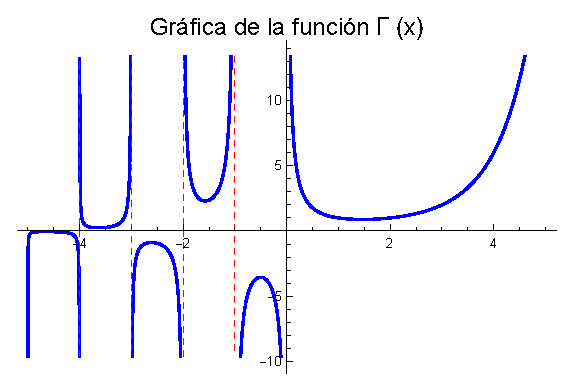
\includegraphics[scale=1]{Imagenes/Plot_Gamma_01.eps}
    \caption{Gráfica de la función Gamma en el intervalo $-5 < x < 5$.}
    \label{fig:figura_02_01}
\end{figure}
\end{frame}
\begin{frame}
\frametitle{El mínimo de la gráfica}
Además, el mínimo ocurre en el intervalo $1 < x < 2$.
\\
\bigskip
\pause
La posición exacta del mínimo fue primero calculada por Gauss y resultó ser $x_{0} = 1.4616\ldots$, \pause lo que lleva al mínimo valor $\Gamma (x_{0}) = 0.8856\ldots$
\end{frame}
\begin{frame}
\frametitle{Resultado importante}
Por último, de la continuidad de $\Gamma (x)$ y su concavidad, deducimos que:
\pause
\begin{align}
\lim_{x \to +\infty} \Gamma (x) \to +\infty
\label{eq:ecuacion_02_13}
\end{align}
\end{frame}
\begin{frame}
\frametitle{Más sobre la gráfica de $\Gamma (x)$}
Con este último resultado, hemos determinado las características fundamentales de la gráfica de la función $\Gamma (x)$ para $x > 0$, como se ve en la figura (\ref{fig:figura_02_01}).
\end{frame}
\begin{frame}[plain]
\begin{figure}[H]
    \centering
    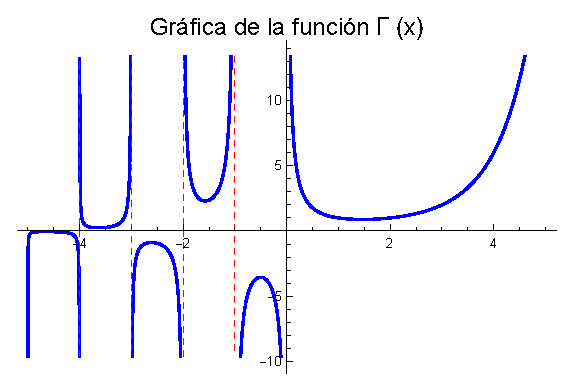
\includegraphics[scale=1.15]{Imagenes/Plot_Gamma_01.eps}
\end{figure}
\end{frame}
\begin{frame}
\frametitle{Manejo de la función $\Gamma (x)$}
La función Gamma se define para valores positivos y negativos de $x$ por la ec. (\ref{eq:ecuacion_02_01}), \pause aunque generalmente es más conveniente utilizar la fórmula de recurrencia (\ref{eq:ecuacion_02_03}) cuando se trata de valores negativos.
\end{frame}
\begin{frame}
\frametitle{Ejemplo para valores negativos}
Por ejemplo, si $x$ está en el rango $-1 < x < 0$, reescribimos la ec. (\ref{eq:ecuacion_02_03}) como:
\pause
\begin{align}
\Gamma (x) = \dfrac{\Gamma (x + 1)}{x} \hspace{1.5cm} x > -1, \hspace{0.5cm} x \neq 0
\label{eq:ecuacion_02_14}
\end{align}
y usamos el lado derecho para fines de cálculo.
\end{frame}
\begin{frame}
\frametitle{Tomando los límites}
También usando la ec. (\ref{eq:ecuacion_02_14}), obtenemos los límites izquierdo y derecho:
\begin{eqnarray*}
\begin{aligned}
\lim_{x \to 0^{-}} \Gamma (x) &= \lim_{x \to 0^{-}} \dfrac{\Gamma (x + 1)}{x} \to -\infty \label{eq:ecuacion_02_15} \\[0.5em] \pause
\lim_{x \to 1^{+}} \Gamma (x) &= \lim_{x \to 1^{+}} \dfrac{\Gamma (x + 1)}{x} \to -\infty \label{eq:ecuacion_02_16}
\end{aligned}
\end{eqnarray*}
\end{frame}
\begin{frame}
\frametitle{Para valores negativos}
Si $(x + 1)$ es aún un número negativo, se puede reemplazar $x$ por $x + 1$ en la ec. (\ref{eq:ecuacion_02_14}) para obtener:
\pause
\begin{align*}
\Gamma (x + 1) = \dfrac{\Gamma (x + 2)}{x + 1}
\end{align*}
\pause
la cual, combinada con la ec. (\ref{eq:ecuacion_02_14}), nos lleva a:
\begin{align*}
\Gamma (x) = \dfrac{\Gamma (x + 2)}{x (x + 1)} \hspace{1cm} x > -2 , \hspace{0.5cm} x \neq 0, -1
\end{align*}
\end{frame}
\begin{frame}
\frametitle{Repitiendo el cálculo}
Continuando con este proceso, se logra la siguiente expresión:
\pause
\begin{align}
\begin{aligned}
\Gamma (x) = \dfrac{\Gamma (x {+} k)}{x (x {+} 1)(x {+} 2) \cdots (x {+} k {-} 1)} \\[0.5em]\hspace{1cm} k = 1, 2, 3, \ldots
\end{aligned}
\label{eq:ecuacion_02_19}
\end{align}
\pause
que define la función Gamma sobre el intervalo $x > -k$ (excepto $x \neq 0, -1, -2, .\ldots , -k + 1)$ en términos de una función Gamma con argumento positivo.
\end{frame}
\begin{frame}
\frametitle{Los límites para otros valores negativos}
De la ec. (\ref{eq:ecuacion_02_19}) vemos que el patrón anterior de límites infinitos alternos en los enteros negativos continúa indefinidamente.
\end{frame}
\begin{frame}[plain]
\begin{figure}[H]
  \centering
  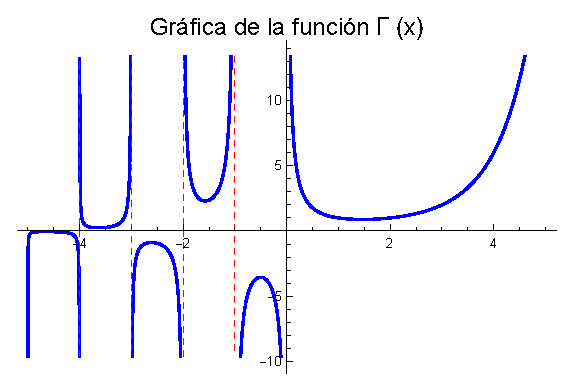
\includegraphics[scale=1.15]{Imagenes/Plot_Gamma_01.eps}
\end{figure}
\end{frame}

\subsection{Otras representaciones integrales}

\begin{frame}
\frametitle{Una representación integral de $\Gamma (x)$}
Además de la expresión:
\pause
\begin{align*}
\scaleint{6ex}_{\bs 0}^{\infty} e^{-t} \, t^{x- 1} \dd{t} \hspace{1cm} x > 0
\end{align*}
hay una variedad de otras representaciones integrales de $\Gamma (x)$, la mayoría de las cuales se pueden obtener de esa mediante simples cambios de variable.
\end{frame}
\begin{frame}
\frametitle{Primer cambio de variable}
Por ejemplo, si hacemos el cambio $t = u^{2}$ en la integral anterior, obtenemos:
\pause
\begin{align}
\Gamma (x) = 2 \scaleint{6ex}_{\bs 0}^{\infty} e^{-u^{2}} \, u^{2x-1} \dd{u} \hspace{1cm} x > 0
\label{eq:ecuacion_02_20}
\end{align}
\end{frame}
\begin{frame}
\frametitle{Otro cambio de variable}
Mientras que el cambio de variable $t = \ln (1/u)$, nos lleva a:
\pause
\begin{align}
\Gamma (x) = \scaleint{6ex}_{\bs 0}^{1} \bigg( \ln \dfrac{1}{u} \bigg)^{x-1} \dd{u} \hspace{1cm} x > 0
\label{eq:ecuacion_02_21}
\end{align}
\end{frame}
\begin{frame}
\frametitle{Expresión más elaborada}
Se puede recuperar una relación un poco más complicada usando la representación que se indica en la ec. (\ref{eq:ecuacion_02_02}) y formando el producto:
\pause
\begin{eqnarray*}
\begin{aligned}
&\Gamma (x) \, \Gamma(y) = 2 \scaleint{6ex}_{\bs 0}^{\infty} e^{-u^{2}} u^{2x-1} \dd{u} \cdot 2 \scaleint{6ex}_{\bs 0}^{\infty} e^{-v^{2}} v^{2y-1} \dd{v} = \\[0.5em] \pause
&= 4 \scaleint{6ex}_{\bs 0}^{\infty} \scaleint{6ex}_{\bs 0}^{\infty} \exp\big( - u^{2} + v^{2} \big) u^{2x-1} v^{2y-1} \dd{u} \dd{v}
\end{aligned}
\end{eqnarray*}
\end{frame}
\begin{frame}
\frametitle{Cambio de variable recomendado}
La presencia del término $u^{2} + v^{2}$ en el integrando sugiere el cambio de variables:
\pause
\begin{align*}
u = r \, \cos \theta \hspace{1cm} v = r \, \sin \theta
\end{align*}
\pause
lo que nos conduce a:
\begin{align*}
\Gamma (x) \, \Gamma (y) &= 4 \scaleint{6ex}_{\bs 0}^{\infty} \scaleint{6ex}_{\bs 0}^{\infty} e^{-r^{2}} \, r^{2x-1} \, \cos^{2x-1} \theta \times \\[0.5em]
&\times r^{2y-1} \, \sin^{2y-1} \theta \, r \dd{r} \dd{\theta} =
\end{align*}
\end{frame}
\begin{frame}
\frametitle{Cambio de variable recomendado}
\begin{eqnarray*}
\begin{aligned}
&= 4 \scaleint{6ex}_{\bs 0}^{\infty} e^{-r^{2}} r^{2(x+y)-1} \dd{r} \cdot \scaleint{6ex}_{\bs 0}^{\frac{\pi}{2}} \cos^{2x-1} \theta \sin^{2y-1} \theta \dd{\theta} = \\[0.5em] \pause
&= 2 \, \Gamma(x + y) \, \scaleint{6ex}_{\bs 0}^{\frac{\pi}{2}} \, \cos^{2x-1} \theta \, \sin^{2y-1} \theta \dd{\theta}
\end{aligned}
\end{eqnarray*}
\end{frame}
\begin{frame}
\frametitle{Resolviendo la integral}
Que al resolver la integral, se obtiene una interesante relación:
\pause
\begin{align}
\begin{aligned}
\scaleint{6ex}_{\bs 0}^{\frac{\pi}{2}} \cos^{2x-1} \theta \, \sin^{2y-1} \theta \dd{\theta} = \dfrac{\Gamma (x) \, \Gamma(y)}{2 \, \Gamma(x + y)} \\[0.5em]
x > 0, y > 0
\end{aligned}
\label{eq:ecuacion_02_22}
\end{align}
\end{frame}
\begin{frame}
\frametitle{Ocupando un valor particular}
Haciendo que $x =  y = 1/2$ en la ec. (\ref{eq:ecuacion_02_22}), se tiene que:
\pause
\begin{align*}
\scaleint{6ex}_{\bs 0}^{\frac{\pi}{2}} \dd{\theta} = \dfrac{\Gamma \bigg( \dfrac{1}{2} \bigg) \, \Gamma \bigg( \dfrac{1}{2} \bigg)}{2 \, \Gamma (1)}
\end{align*}
\pause
de donde se obtiene el valor especial:
\pause
\begin{align}
\Gamma \bigg( \dfrac{1}{2} \bigg) = \sqrt{\pi}
\label{eq:ecuacion_02_23}
\end{align}
\end{frame}

\section{Ejemplos}
\frame{\tableofcontents[currentsection, hideothersubsections]}
\subsection{Ejercicio 1}

\begin{frame}
\frametitle{Ejercicio 1}
Evaluar la integral:
\pause
\begin{align*}
\scaleint{6ex}_{\bs 0}^{\infty} x^{4} \, e^{-x^{3}} \dd{x}
\end{align*}
\end{frame}
\begin{frame}
\frametitle{Haciendo el cambio de variable}
Hagamos que $t = x^{3}$, para así expresar la integral como:
\pause
\begin{eqnarray*}
\begin{aligned}
\scaleint{6ex}_{\bs 0}^{\infty} x^{4} \, e^{-x^{3}} \dd{x} &= \pause \dfrac{1}{3} \, \scaleint{6ex}_{\bs 0}^{\infty} e^{-t} \, t^{\frac{2}{3}} \dd{t} = \\[0.5em] \pause
&= \dfrac{1}{3} \, \Gamma \bigg( \dfrac{5}{3} \bigg) = \\[0.5em]
&= 0.300915
\end{aligned}
\end{eqnarray*}
\end{frame}

\subsection{Ejercicio 2}

\begin{frame}
\frametitle{Ejercicio 2}
Demuestra la expresión asintótica:
\pause
\begin{align*}
\Gamma (x + 1) \thicksim \sqrt{2 \, \pi \, x} \, x^{x} e^{-x} \hspace{1.5cm} x \to \infty
\end{align*}
\end{frame}
\begin{frame}
\frametitle{Resolviendo el Ejercicio 2}
Haciendo el cambio de variable $t = x + s$ en la representación integral:
\pause
\begin{align*}
\Gamma (x + 1) = \scaleint{6ex}_{\bs 0}^{\infty} t^{x} \, e^{-t} \dd{t}
\end{align*}
\pause
se obtiene:
\begin{align*}
\Gamma (x + 1) = x^{x} \, e^{-x} \scaleint{6ex}_{\bs -x}^{\infty} \exp\bigg[ x \, \ln \bigg( 1 + \dfrac{s}{x} \bigg) \bigg] \, e^{-s} \dd{s}
\end{align*}
\end{frame}
\begin{frame}
\frametitle{Considerando valores grandes de $x$}
Para valores grandes de $x$, podemos usar la aproximación:
\pause
\begin{align*}
\ln \bigg( 1 + \dfrac{s}{x} \bigg) \thicksim \dfrac{s}{x} - \dfrac{s^{2}}{2 \, x^{2}} \hspace{1cm} x \to \infty
\end{align*}
\pause
Recordemos que:
\begin{align*}
\ln (1 + x) = \nsum_{n=0}^{\infty} (-1)^{n} \, \dfrac{x^{n+1}}{n + 1}
\end{align*}
\end{frame}
\begin{frame}
\frametitle{Ocupando la aproximación}
Lo que nos conduce a:
\pause
\begin{eqnarray*}
\begin{aligned}
\Gamma (x + 1) &\thicksim x^{x} \, e^{-x} \scaleint{6ex}_{\bs -\infty}^{\infty} \exp\bigg( -\dfrac{s^{2}}{2 \, x} \bigg) \dd{s} \\[0.5em] \pause
&\thicksim \sqrt{2 \, x} \, x^{x} \, e^{-x} \, \scaleint{6ex}_{\bs -\infty}^{\infty} e^{-u^{2}} \dd{u}
\end{aligned}
\end{eqnarray*}
En este último paso, se ha hecho el cambio de variable $u = s / \sqrt{2 x}$.
\end{frame}
\begin{frame}
\frametitle{Cambio de variable necesario}
Usando las propiedades de las funciones pares y recordando las ecs. (\ref{eq:ecuacion_02_20}) y (\ref{eq:ecuacion_02_23}), esta última integral da:
\pause
\begin{eqnarray*}
\begin{aligned}
\scaleint{6ex}_{\bs -\infty}^{\infty} e^{-u^{2}} \dd{u} &= 2 \, \scaleint{6ex}_{\bs 0}^{\infty} e^{-u^{2}} \dd{u} = \\[0.5em] \pause
&= \Gamma \bigg( \dfrac{1}{2} \bigg) = \\[0.5em]
&= \sqrt{\pi}
\end{aligned}
\end{eqnarray*}
\end{frame}
\begin{frame}
\frametitle{Recuperando los resultados}
Combinando los resultados, se deduce entonces que:
\pause
\begin{align*}
\Gamma (x + 1) \thicksim \sqrt{2 \, \pi \, x} \, x^{x} e^{-x} \hspace{1.5cm} x \to \infty
\end{align*}
que es conocida como la \textbf{fórmula de Stirling}.
\end{frame}
\begin{frame}
\frametitle{Comparando con respecto al factorial}
El cálculo de valores del factorial de $x$ ocupando la fórmula de Stirling será siempre una aproximación que estará por debajo del factorial cuando se calculan valores pequeños de $x$, \pause mientras que se tiende a reducir la diferencia para valores mayores de $x$.
\end{frame}
\begin{frame}
\frametitle{Ejemplo de cálculo}
En la siguiente tabla se presenta un ejemplo, mediante el cálculo directo del factorial $n!$ y mediante la fórmula de Stirling $s(n)$ y el error relativo entre estos valores:
\end{frame}
\begin{frame}
\frametitle{Tabla de valores}
\begin{table}[H]
\centering
\begin{tabular}{l l l l}
$n$ & $n!$ & $s(n)$ & $\mbox{error}_{\mbox{rel}}$ \\ \hline
$1$ & $1$ & $0.92213$ & $7.7863$ \\ \hline \pause
$2$ & $2$ & $1.919$ & $4.0497$ \\ \hline \pause
$3$ & $6$ & $5.8362$ & $2.7298$ \\ \hline \pause
$4$ & $24$ & $23.5062$ & $2.0576$ \\ \hline
$5$ & $120$ & $118.019$ & $1.65069$
\end{tabular}
\end{table}
\end{frame}
\begin{frame}
\frametitle{Tabla de valores}
\begin{table}[H]
\centering
\begin{tabular}{l l l l}
$n$ & $n!$ & $s(n)$ & $\mbox{error}_{\mbox{rel}}$ \\ \hline
$6$ & $720$ & $710.078$ & $1.37803$ \\ \hline \pause
$7$ & $5040$ & $4980.4$ & $1.18262$ \\ \hline \pause
$8$ & $40320$ & $39902.4$ & $1.03573$ \\ \hline \pause
$9$ & $362880$ & $359537$ & $0.921276$ \\ \hline
\end{tabular}
\end{table}
\end{frame}
\begin{frame}
\frametitle{Tabla de valores}
\begin{table}[H]
\centering
\begin{tabular}{l l l l}
$n$ & $n!$ & $s(n)$ & $\mbox{error}_{\mbox{rel}}$ \\ \hline
$10$ & $3628800$ & $\num[tight-spacing=true]{3.5987d6}$ & $0.829596$ \\ \hline \pause
$15$ & $\num[tight-spacing=true]{1.3076d12}$ & $\num[tight-spacing=true]{1.30043d12}$ & $0.553933$ \\ \hline \pause
$20$ & $[19]$ dígitos & $\num[tight-spacing=true]{2.42279d18}$ & $0.415765$ \\ \hline \pause
$100$ & $[158]$ dígitos & $\num[tight-spacing=true]{9.32485d157}$ & $0.083298$ \\ \hline \pause
$\num{e4}$ & $[35660]$ dígitos & $\num[tight-spacing=true]{2.84624d35659}$ & $0.0$ \\ \hline
\end{tabular}
\end{table}
\end{frame}

\subsection{Ejercicio 3}

\begin{frame}
\frametitle{Ejercicio 3}
Para $x > 0$ calcula el área entre:
\begin{align*}
y = 4 x^{\frac{3}{2}} \, \exp \bigg( - \dfrac{x^{2}}{2} \bigg)
\end{align*}
y su asíntota.
\end{frame}
\begin{frame}
\frametitle{Gráfica de la función}
\begin{figure}
  \centering
  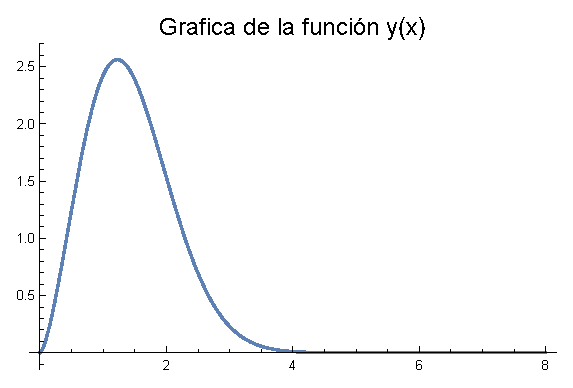
\includegraphics[scale=1]{Imagenes/Plot_Gamma_02_Ejercicio.eps}
\end{figure}
\end{frame}
\begin{frame}
\frametitle{Resolviendo el ejercicio}
A partir de la figura anterior es claro que la curva se encuentra completamente por encima del eje $x$ positivo con el eje $x$ actuando como una asíntota cuando $x \to \infty$.
\end{frame}
\begin{frame}
\frametitle{Calculando el área debajo de la curva}
Por lo tanto, el área bajo la curva viene dada por la fórmula estándar:
\pause
\begin{eqnarray*}
A = \scaleint{6ex}_{\bs 0}^{\infty} y \dd{x} = \pause 4 \scaleint{6ex}_{\bs 0}^{\infty} x^{\frac{3}{2}} \, \exp\bigg( -\dfrac{x^{2}}{2} \bigg) \dd{x}
\end{eqnarray*}
\end{frame}
\begin{frame}
\frametitle{Cambiando la variable}
Haciendo el cambio de variable $t = x^{2} / 2$, se tiene que:
\pause
\begin{eqnarray*}
\begin{aligned}
A &= 2^{\frac{9}{4}} \scaleint{6ex}_{\bs 0}^{\infty} t^{\frac{1}{4}} \, e^{-t} \dd{t} = \\[0.5em] \pause
&= 2^{\frac{9}{4}} \, \Gamma \bigg( \dfrac{5}{4} \bigg) = \\[0.5em] \pause
&= 4.3116 \hspace{1.5cm} \qed
\end{aligned}
\end{eqnarray*}
\end{frame}
\end{document}